\documentclass{beamer}
\usetheme[progressbar=frametitle]{metropolis}
\usepackage[font=small,labelfont=bf,tableposition=top]{caption}
\usepackage{listings}

\lstdefinestyle{mystyle}{
    % backgroundcolor=\color{backcolour},   
    % commentstyle=\color{codegreen},
    % keywordstyle=\color{magenta},
    % numberstyle=\tiny\color{codegray},
    % stringstyle=\color{codepurple},
    basicstyle=\ttfamily\footnotesize,
    % breakatwhitespace=false,         
    % breaklines=true,                 
    % captionpos=b,                    
    % keepspaces=true,                 
    % numbers=left,                    
    % numbersep=5pt,                  
    % showspaces=false,                
    % showstringspaces=false,
    % showtabs=false,                  
    % tabsize=2
}

\lstset{style=mystyle}

\title{Baking Egg into Souffl\'e}
\subtitle[]{Building compiler optimizations in Datalog}
\author{\textbf{Remy Wang}, Yihong Zhang, Max Willsey, Philip Zucker, Zachary Tatlock }
\date{April 2022 @ HYTRADBOI}

\begin{document}

\frame{\titlepage}

\begin{frame}
    \frametitle{How does a compiler optimize?}
    \begin{figure}
        \includegraphics<1>{searchspace1.pdf}%
        \includegraphics<2>{searchspace2.pdf}%
        \includegraphics<3>{searchspace3.pdf}%
        \includegraphics<4>{searchspace4.pdf}%
        \includegraphics<5->{searchspace5.pdf}%
    \end{figure}
    Cascade style\footnote{A.k.a.\ equality saturation.}: 
     explore the space of equivalent programs.
    
    \uncover<6>{Main loop: match rewrite rules on programs to grow the set.}
\end{frame}

% \begin{frame}
%     \frametitle{How does a compiler optimize?}
%     Compact representation of equivalent programs:
%     \begin{figure}
%         \visible<1->{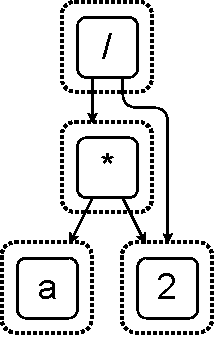
\includegraphics[height=0.3\textheight]{egraph1.pdf}}
%         \visible<2->{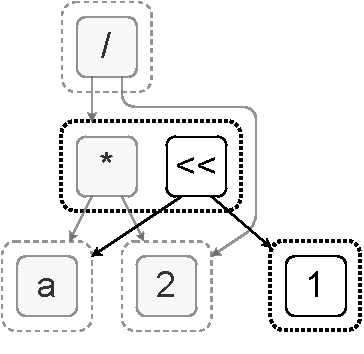
\includegraphics[height=0.3\textheight]{egraph2.pdf}}
%         \visible<3->{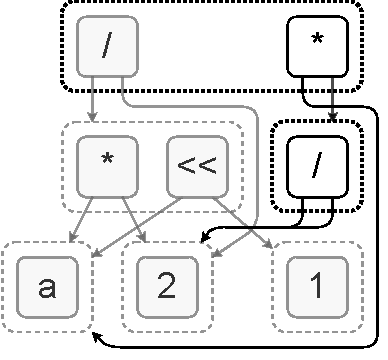
\includegraphics[height=0.3\textheight]{egraph3.pdf}}
%         \visible<4->{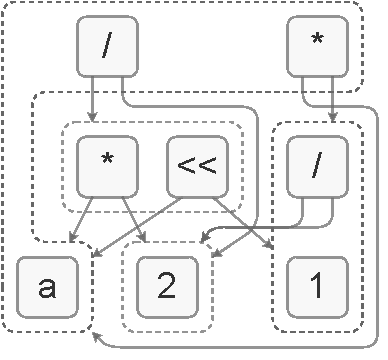
\includegraphics[height=0.3\textheight]{egraph4.pdf}}
%     \end{figure}
%     Group equivalent subexpressions into \textbf{equivalent classes}.

%     \uncover<5>{Main loop: match rewrite rules on programs to grow the set.}
% \end{frame}

\begin{frame}
    \frametitle{How does a compiler optimize?}
    
    Main \textbf{loop}: \textbf{match} rewrite \textbf{rules} on programs to \textbf{grow the set}. \pause

    Datalog does that all day, every day!
\end{frame}

\begin{frame}[fragile]
    \frametitle{Optimization in Datalog: Encoding Terms}
    ``Flat'' representation of terms:
    \begin{figure}
        \raisebox{-.5\height}{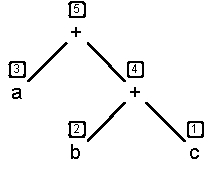
\includegraphics{ast.pdf}}
        \, $\Rightarrow$ \,%
        \begin{tabular}{ c c }
            $var$ & $id_{var}$ \\
            \hline
             c & 1 \\ 
             b & 2\\
             a & 3
        \end{tabular}
        \quad
        \begin{tabular}{ c c c }
        $arg_1$ & $arg_2$ & $id_+$ \\
        \hline
            2 & 1 & 4\\ 
            3 & 2 & 5
        \end{tabular}
    \end{figure} %
    \pause

    In Souffl\'e:
    \begin{lstlisting}[language=Python]
.decl add(x:number,y:number,id:number)
.decl var(v:symbol,id:number)
    \end{lstlisting}
%     \begin{lstlisting}[language=Python]
% .type Exp = Add{x:Exp,y:Exp} | Var{n:symbol}
% .decl add(x:Exp,y:Exp,id:Exp)
% .decl var(v:symbol,id:Exp)
% add(x,y,id) :- id=$Add(x,y).
%     \end{lstlisting}
\end{frame}

\begin{frame}[fragile]
    \frametitle{Optimization in Datalog: Encoding Terms}
    Group equivalent subexpressions into \textbf{equivalence classes}:
    \begin{figure}
        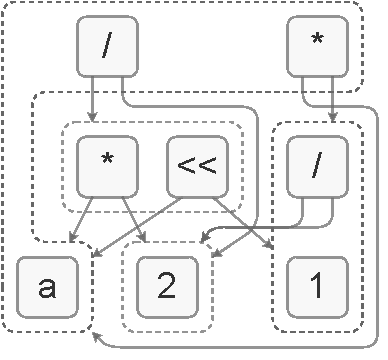
\includegraphics[height=0.4\textheight]{egraph4.pdf}
    \end{figure}
    \pause
    \begin{lstlisting}[language=Python]
.decl eql(x:number,y:number) eqrel
// keep only canonical term
add(x,y,z) <= add(a,b,c) :-
    eql(x,a), eql(y,b), eql(z,c),
    a<=x, b<=y, c<=z.
    \end{lstlisting}
%     \begin{lstlisting}[language=Python]
% .decl eql(x:Exp,y:Exp) eqrel
% // keep only canonical Exp
% add(x,y,z) <= add(a,b,c) :-
%   eql(x,a), eql(y,b), eql(z,c),
%   a<=x, b<=y, c<=z.
%     \end{lstlisting}
\end{frame}

\begin{frame}[fragile]
    \frametitle{Optimization in Datalog: Encoding Rewrites}
     A rewrite can add new terms and new equalities~\footnote{A.k.a.\ tgds and egds.}:
     \begin{lstlisting}[language=Python]
// comm-add
eql(xy,yx), add(x,y,xy) :- 
    add(y,x,yx), xy=@hash('+',x,y).
    \end{lstlisting}
    \pause
    \begin{lstlisting}[language=Python]
// assoc-add
eql(xy_z,x_yz), add(xy,z,xy_z), add(x,y,xy) :-
    add(y,z,yz), add(x,yz,x_yz),
    xy=@hash('+',x,y), xy_z=@hash('+',xy,z).
    \end{lstlisting}
%      \begin{lstlisting}[language=Python]
% // comm-add
% eql(xy,yx), add(x,y,xy) :- 
%   add(y,x,yx), xy=$Add(x,y).
%     \end{lstlisting}
%     \pause
%     \begin{lstlisting}[language=Python]
% // assoc-add
% eql(xy_z,x_yz), add(xy,z,xy_z), add(x,y,xy) :-
%   add(y,z,yz), add(x,yz,x_yz),
%   xy = $Add(x,y), xy_z = $Add(xy,z).
%     \end{lstlisting}
\end{frame}

\begin{frame}[fragile]
    \frametitle{Optimization in Datalog: Picking the Best Term}
     Analyzing cost is very natural:
     \begin{lstlisting}[language=Python]
.decl n_cost( node:number, c:number) // cost of node
.decl c_cost(class:number, c:number) // cost of class

n_cost(xy,a+b+1) :- add(x,y,xy), c_cost(x,a), c_cost(y,b).
n_cost(v,1) :- var(v,_).

c_cost(x,c) :- eq(x,y), n_cost(y,c).
c_cost(x,a) <= c_cost(x, b) :- a >= b.
    \end{lstlisting}
\end{frame}

\begin{frame}
    \frametitle{Optimization in Datalog: What's the Point?}
    \textbf{Performance:}
    \begin{itemize}
        \item Join algorithms for e-matching~\cite{ZhangWWT22}.
        \item Semi-na\"ive/IVM (TreeToaster~\cite{BalakrishnanNKZ21})
    \end{itemize}
    \pause
    \textbf{Expressiveness:}
    \begin{itemize}
        \item Composable lattice-style program analyses (Flix~\cite{MadsenYL16})
        \item Leverage existing analysis (DOOP~\cite{BravenboerS09})
    \end{itemize}
\end{frame}

\begin{frame}
    \frametitle{Optimization in Datalog: What's Left?}
    \textbf{Performance:}
    \begin{itemize}
        \item Actually efficient equivalence relation (\texttt{eqrel} in Souffl\'e~\cite{NappaZSS19}).
        \item Congruence algorithms~\cite{WillseyNWFTP21} (semi-na\"ive?).
    \end{itemize}
    \pause
    \textbf{Expressiveness:} what to do with this new-found power??
    \begin{itemize}
        \item Improve precision of analyses~\cite{Steensgaard96}?
        \item Composing transformation \& analyses\cite{LernerGC02}?
        \item Decompiler~\cite{GrechBSS19}?
        \item Relations other than equivalence (e.g. implication)?
        \item ...
    \end{itemize}
\end{frame}

\begin{frame}[allowframebreaks]
    \frametitle{References}
    \bibliographystyle{amsalpha}
    \bibliography{main.bib}
\end{frame}

\end{document}
